%
% Modo de operación CFB, capítulo de antecedentes.
% Proyecto Lovelace.
%

\subsubsection{\texorpdfstring{\acrfull{gl:cfb}}{Cipher Feedback (CFB)}}

Al igual que la operación de cifrado de \gls{gl:cbc}, ambas operaciones
de \gls{gl:cfb} (cifrado y descifrado) están encadenadas bloque a bloque,
por lo que son de naturaleza secuencial. En este caso, lo que se cifra en el
primer paso es el \gls{gl:vector_de_inicializacion}; la salida de esto se opera
con un \verb|xor| sobre el primer bloque de texto en claro, para obtener el
primer bloque cifrado (figura~\ref{fig:cfb}).

Esta distribución presenta varias ventajas con respecto a \gls{gl:cbc}:
las operaciones de cifrado y descifrado son sumamente similares, lo que permite
ser implementadas por un solo algoritmo (pseudocódigo~\ref{cfb:1}); tanto para
cifrar como para descifrar solamente se ocupa la operación de cifrado del
algoritmo a bloques subyacente. Estas ventajas se deben principalmente a las
propiedades de la operación \verb|xor| (ecuación~\ref{xor:inverso_igual}).
\begin{equation}
  \label{xor:inverso_igual}
  A \oplus B = C \quad \Rightarrow \quad A = B \oplus C
\end{equation}

\begin{figure}
  \centering
  \begin{subfigure}{0.45\textwidth}
    \begin{center}
      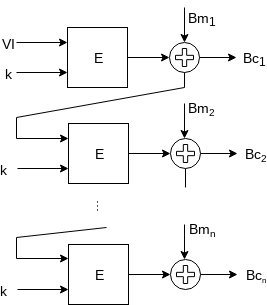
\includegraphics[width=0.6\linewidth]{diagramas/modo_cfb.png}
      \caption{Cifrado.}
    \end{center}
  \end{subfigure}
  \begin{subfigure}{0.45\textwidth}
    \begin{center}
      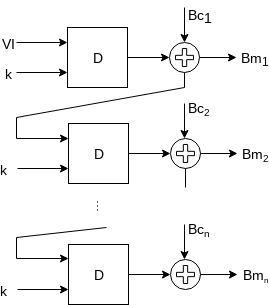
\includegraphics[width=0.6\linewidth]{diagramas/modo_cfb_inverso.png}
      \caption{Descifrado.}
    \end{center}
  \end{subfigure}
  \caption{\Gls{gl:modo_de_operacion} \acrshort{gl:cfb}.}
  \label{fig:cfb}
\end{figure}

\begin{pseudocodigo}[%
    caption={\Gls{gl:modo_de_operacion} \acrshort{gl:cfb}%
      (cifrado y descifrado).},
    label={cfb:1}%
  ]
    entrada: llave $ k $; vector de inicialización $ VI $;
             bloques de mensaje (cifrado o descifrado) $ Bm_1, Bm_2 \dots Bm_n $.
    salida:  bloques de mensaje (cifrado o descifrado) $ Bc_1, Bc_2 \dots Bc_n $.
    inicio
      $Bc_0$ $\gets$ $ VI $
      para_todo $Bm$
        $Bc_i$ $\gets$ $C_k$($Bc_{i - 1}$) $\oplus$ $Bm_i$
      fin
      regresar $Bc$
    fin
\end{pseudocodigo}
